\documentclass{article}
\usepackage[spanish]{babel} %Definir idioma español
\usepackage[utf8]{inputenc} %Codificacion utf-8
\usepackage{amssymb, amsmath, amsbsy, wasysym}
\usepackage{multirow} % para tablas
\usepackage{graphicx}
\usepackage[dvipsnames]{xcolor}
\title{Práctica 5}
\author{Emmanuel Peto Gutiérrez}
\begin{document}
\maketitle

\section{Introducción}

Esta práctica consiste en implementar un algoritmo que identifique las componentes conexas de una gráfica $G$, dicho algoritmo puede ser implementado de dos formas, utilizando {\bf BFS} o {\bf DFS}.

\section{Descripción}

\subsection{Entrada}

El programa recibe como entrada el nombre del archivo de texto que contiene la información necesaria para construir la gráfica $G$. Esto es:\\
$\bullet$ En la primer linea, los vértices de la gráfica separados por coma.\\
$\bullet$ De la segunda línea en adelante, pares de vértices separados por coma que indican las aristas de la gráfica.

En este caso, los vértices se van a representar con números.

\subsection{Salida}

El programa debe imprimir en consola cada una de las componentes conexas, separadas por un salto de línea.

Por ejemplo, para la gráfica:

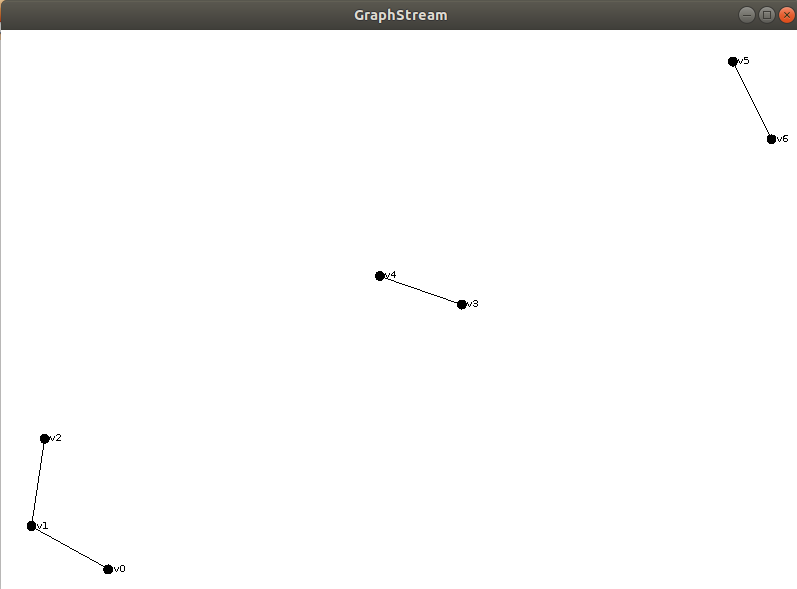
\includegraphics[scale=0.2]{3component}

el resultado debe ser:

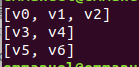
\includegraphics[scale=1]{3component_terminal}

\section{Extra}

Al aplicar los algoritmos {\bf BFS} o {\bf DFS} se genera un árbol, o un bosque si no es conexa. Se obtendrá un punto extra si pintan de rojo a las aristas que pertenecen al bosque y de negro las que no.

\section{Entrega}

\begin{itemize}
\item Deben entregarlo como un archivo comprimido de una carpeta con el mismo nombre.
\item La carpeta debe ser: \textbf{Practica5\_ApellidopaternoApellidomaterno}. Por ejemplo \textbf{Practica5\_PetoGutierrez}.
\item Su carpeta debe contener un archivo \emph{readme} que contenga: número de cuenta, nombre completo, 
correo y las instrucciones para compilar y ejecutar su programa(se recomienda un \emph{Makefile}).
\item Si su carpeta contiene un ejecutable(como *.jar) enviarlo como un enlace de dropbox o drive.
\item El asunto debe ser: \textbf{[AAlgoritmos]Practica5}.
\item El correo al que enviarán la práctica es: \emph{empg014@ciencias.unam.mx}
\end{itemize}

La fecha de entrega es el \textbf{6 de noviembre}.

\end{document}


